\chapter{Einleitung}
\label{text:einleitung}
Magnetische Domänen stellen ein großes Interesse in dem Bereich von Festkörperphysik dar. Zum Durchführen der Streuexperimentean an den mikroskopischen magnetischen Strukturen wird die Röntgenstrahlung verwendet. Die vorausgesetzten Anforderungen an die Kohärenz und Brillanz der Quelle können hauptsächlich nur mithilfe von speziellen Anlagen wie Synchrotron oder Freie-Elektronen-Laser erfüllt werden. Limitierte Kapazität, technische Komplexität und Einzigartigkeit solcher Anlagen bestimmt (legt fest) eine (strikte) zeitliche Grenze, innerhalb deren ein Experiment durchgeführt werden kann. Unter anderem (Darüber hinaus) tauchen die zusätzlichen Anforderungen in Form von zeitaufwendiger Einarbeitung und pausenlosem mehrtägigem Einsatz der Mitarbeiter auf.

\noindent
Davon ausgehend, wäre die Möglichkeit bevorzugt, diese Art von Experimenten im Labor durchzuführen. Die vergleichbaren Strahlungscharakteristiken  sind allerdings mit den existierenden Röntgenquellen im Labor nicht erreicht. Da es bisher technisch bedingt nicht realisierbar ist, können die Messergebnisse durch die neuen Mess- und Auswertungsmethoden verbessert werden.

%weiche röntgenstrahlung, kleiner Flux -> kleiner Kontrast
\noindent
Das Ziel dieser Arbeit ist so ein Mess- und Auswertungsverfahren mit dem Einsatz der Kurzpulsquelle weicher Röntgenstrahlung anzubieten (herauszufinden), in dem man einzelne Photonen in einem Streubild detektieren und die von Hintergrundrauschen des Bildes (ab)trennen kann. Eine besondere Herausforderung 
MOTIVATION SINGLE PHOTON COUNTING

Idee: für die höhere x-ray Energien ist es möglich die Photonen von dem Rauschen mit einem Komporator (x > threshold) zu trennen. In dem Weichröntgenbereich ist es nicht möglich. Die Innovation liegt daran:  einzelne Photonen in den Aufnahmen mit ultrakurzen Belichtungszeiten zu erkennen, was in Verbindung mit einer hervorragend kurzen Auslesezeit des Detektors ermöglicht, die rauschenlosen Aufnahmen zu bekommen.

% Ich habe noch ganz vergessen, was zu deinem Inhaltsverzeichnis des Theorieteils deiner Arbeit zu sagen. Im Prinzip hast du die richtigen Themen erkannt. Ich würde etwas weiter einengen:
% 1. Resonante Röntgenstreuung von mesoskopischen magnetischen Texturen – bitte lass uns rechtzeitig darüber reden, was da genau rein soll.
% 2. Laser-getriebenes Instrument für resonante Streuung mit weichen Röntgenstrahlen – hier benötigst du fast ausschließlich das Paper von Daniel (https://www.osapublishing.org/optica/abstract.cfm?uri=optica-8-9-1237). Einfach die technischen Details zusammenfassen.
% 3. Der MÖNCH-Detektor – Hier bitte die Paper von den PSI-Leuten nutzen. Nicht zu viel allgemeines, lieber genau den MÖNCH-Detektor erklären.
% 4. Droplet Algorithmen – kurze Übersicht und dann genauer ein Algorithmus, den du ausprobieren möchtest.
% e Qualität bietet sich das Signal-Rausch-Verhältnis (engl. signal-to-noise-ratio, kurz: SNR) 

\chapter{Prinzipien der magnetischen Resonanzstreuung}
\label{text:streuung}
In diesem Kapitel werden die Aspekte der magnetischen Streuung erläutert, um besseres Verständnis und Motivation zur Wahl des Experimentaufbaus dadurch zu bringen. Die Theorie basiert sich auf hauptsächlich \cite{kortright_resonant_2013}. 


\noindent
Die Streuung an einem Element wird durch den elementspezifischen atomaren Streufaktor
\begin{align}
f(h\nu) = (\mathbf{\hat{e}_f^*} \cdot \mathbf{\hat{e}_0})f_c - i(\mathbf{\hat{e}_f^*} \times \mathbf{\hat{e}_0})\cdot\mathbf{\hat{m}}f_{m1}+(\mathbf{\hat{e}_f^*} \cdot \mathbf{\hat{m}})(\mathbf{\hat{e}_0}\cdot\mathbf{\hat{m}})f_{m2} + \dots
\end{align}
beschrieben, wobei $\hat{e}_f^*$ und $\hat{e}_0$ - die einfallenden und auslaufenden normierten Polarisationsvektoren, $\hat{m}$ - der Einheitsvektor entlang der Magnetisierungsachse und $f_c, f_{m1}, f_{m2}$ - die konstanten Streukoeffizienten von Atom. Für den Photonenergiebereich $h\nu$, der weit von der Resonanzabsorptionsfrequenz des Elements liegt, sind die Streukoeffizienten  $f_{m1}, f_{m2}$ klein gegen $f_c$ und werden daher vernachlässigt. Aus diesem Grund hängt der Streufaktor $f(h\nu)$ in dem Bereich lediglich von den Polarisationsvektoren $\hat{e}_f^*$ und $\hat{e}_0$ ab.

\noindent
Im Photonenenergiebereich $h\nu$, der nah an der Resonanzabsorptionsfrequenz des Elements liegt, nehmen die Streukoeffizienten $f_{m1}, f_{m2}$ zu und leisten den dominierenden Beitrag zum Gesamtwert des Streufaktors $f(h\nu)$ bei. Es ist auch wichtig zu beachten, dass der Streufaktor $f(h\nu)$ nun auch von der räumlichen Ausrichtung der Magnetisierungsachse $\hat{m}$ in Bezug auf $\hat{e}_f^*$ und $\hat{e}_0$ abhängt.
\begin{figure}
    \centering
    \input{wellenvektoren.pdf_tex}
    \caption{Caption}
    \label{fig:my_label}
\end{figure}
\noindent
Betrachtet wird der 
%  Kurze Einleitung, wie man die Röntgenstrahlung durch Belichten eines wolframzylinders bekommt (verweis auf TU-Paper). DAS SPEKTRUM von Pape
% \section{Resonante Röntgenstreuung von mesoskopischen magnetischen Texturen}
Die Probe ist nach dem Rezept \cite{tripathi_dichroic_2011} hergestellt. MFM Bilder, Simulation mit \cite{schick_udkm1dsim_2021}.
\begin{figure}[h]
    \centering
    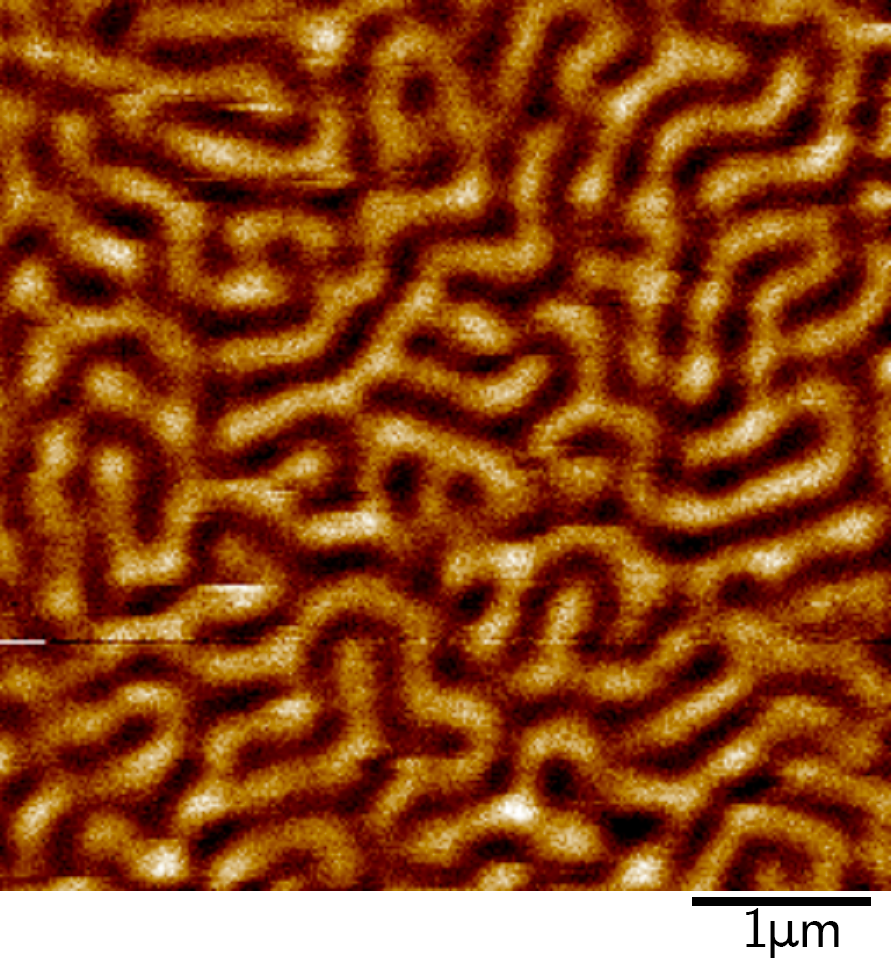
\includegraphics[width=0.25\textwidth]{images/ds220126_R1_membrane_amplitude_cropped.png}
    \caption{Die aufgenommenen Domäne von der Probe. Aufgenommen mit dem Bruker Dimension Icon$^{\text{®}}$ Rastermikroskop im MFM Modus.}
    \label{fig:mfm_amplitude}
\end{figure}
%„ “

\newpage